\section{Coefficients}

\begin{figure}[H]
	\centering
	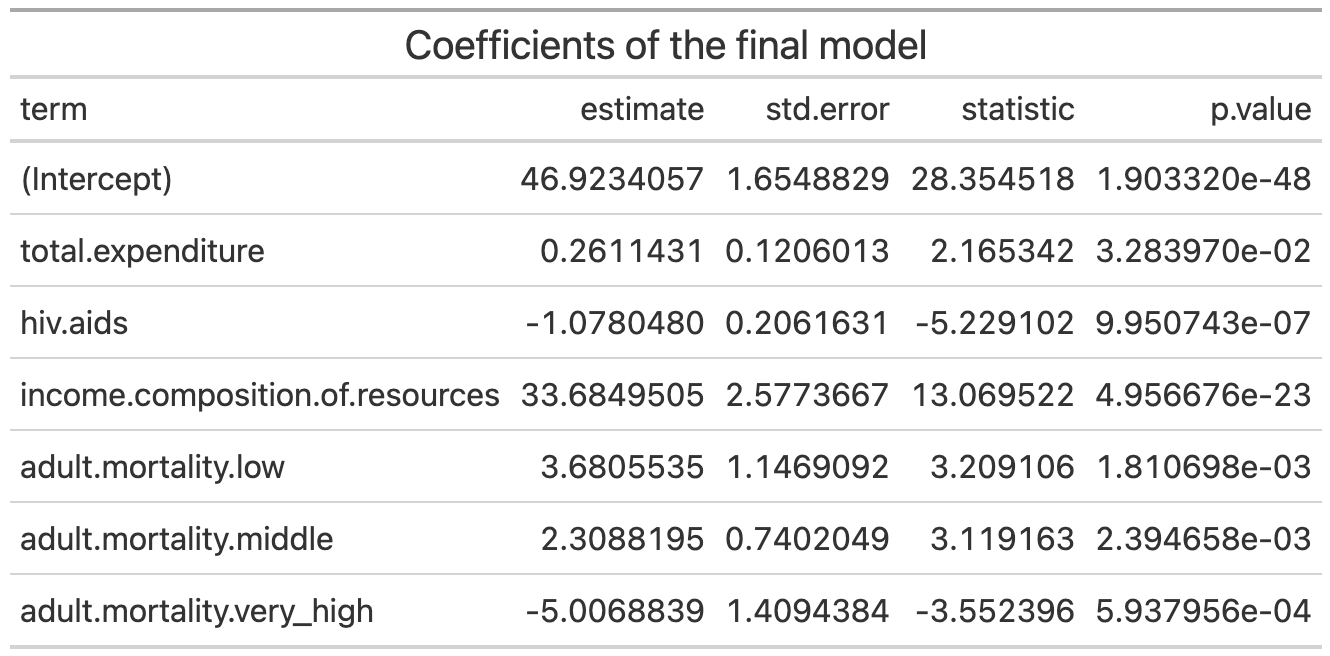
\includegraphics{figures/coefficients/coeff-model.png}
	\caption{Coefficients of the model}
	\label{fig:coeff-model}
\end{figure}

Looking at the p-values, all the coefficients $\beta_k$ are statistically significants at a significance level of $\alpha = 0.05$.

We can interpret the different coefficients the following way,
\begin{itemize}
	\item An increase of $1\%$ in the governement expenditure on health (as a percentage of total expenditure) leads to an increase of $0.26\%$ of life expectancy.
	\item An increase of $1$ death caused by HIV/AIDS for people under $5$ years old per $1000$ births leads to a decrease of $1.07/1000$ of life expectancy.
	\item An increase of ...
	\item Having a low adult mortality leads to an incrase of $3.6$ years of life expectancy.
	\item Having a middle adult mortalty leads to an increase of $2.3$ years of life expectancy.
	\item Having a very high adult mortality leads to a decrease of $5$ years of life expectancy.
\end{itemize}


\section{Significance of estimated coefficients}

We perform t-tests of estimated coefficients in order to test their significance. For t-tests, we use the following null and alternative hypotheses for each regression coefficient: 
\begin{align*}
	H_0&: \beta_i = 0 \\
	H_1&: \beta_i \neq 0
\end{align*}

\begin{figure}[H]
	\centering
	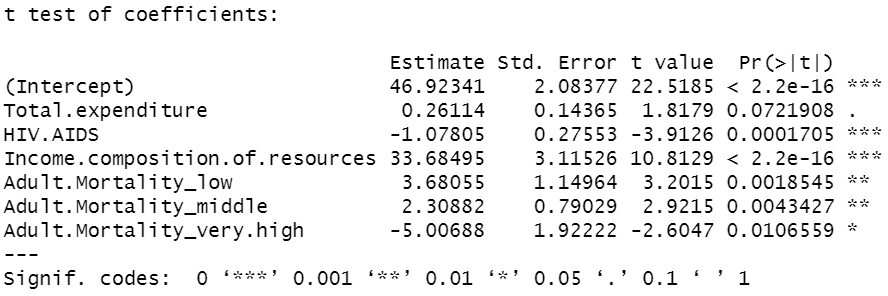
\includegraphics{figures/hypothesis_testing/test_t_coefficients_robust_inference.PNG}
	\caption{Output of t-test of coefficients}
\end{figure}

On the basis of the p-values, we can reject the null hypothesis for all the coefficients. We can conclude that all the coefficients are statistically significant at a level of significance of $10\%$. At a significance level of $5\%$, the “total expenditure” coefficient is no longer statistically significant. \\

On the basis of the estimates, we can say that the effect of low and middle adult mortality rates on life expectancy are positive while the effect of a very high adult mortality rate on life expectancy is negative and stronger. From the regression output, we see that the estimate of the regression coefficient for “Adult mortality very high” is -5.007. This signifies that on average, a country with a very high adult mortality rate has a life expectancy of 5 years less. On the contrary, a country with a low  adult mortality rate has a life expectancy higher of 3 years on average and 2 years for a country with a moderate adult mortality rate. 

\section{Linear combination  of coefficients}

 We want to test the hypothesis that there exists a linear combination between two regression coefficients: 
 \begin{equation*}
     \beta_4 = \beta_5
 \end{equation*} 

 With this, we want to test if these two coefficients are equal. We can also write it as follow: \begin{equation*}
     \beta_4 - \beta_5 = 0
 \end{equation*}

We formulate the null and alternative hypotheses : 
\begin{align*}
	H_0&: \beta_4 - \beta_5 = 0 \\
	H_1&: \beta_4 - \beta_5 \neq 0
\end{align*}

\begin{figure}[H]
	\centering
	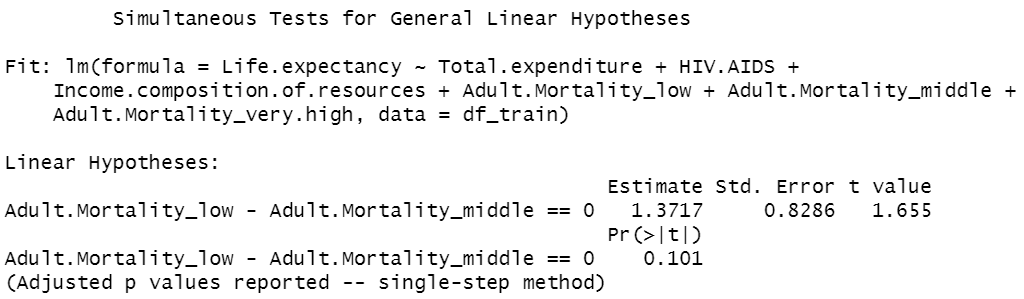
\includegraphics{figures/hypothesis_testing/linear_combination_of_coeff.PNG}
	\caption{Output of linear combination test}
\end{figure}

Since the p-value (0.101) is larger than the significance level of 0.05, we fail to reject the null hypothesis that these two regression coefficients are equal. This signifies that a country with a low adult mortality rate and a country with a moderate adult mortality rate could have the same reduction in years of life expectancy if all the other effects remain constant. 

\section{Coefficients equal to zero}

We test a subset of coefficients equal to zero. In this case, we test the coefficients corresponding to all qualitative variables equal to zero. Hence, the null and alternative hypotheses are the following :

\begin{align*}
	H_0&: \beta_4 = \beta_5 = \beta_6 = 0 \\
	H_1&: \text{at least one of these is not equal to zero}
\end{align*}

\begin{figure}[H]
	\centering
	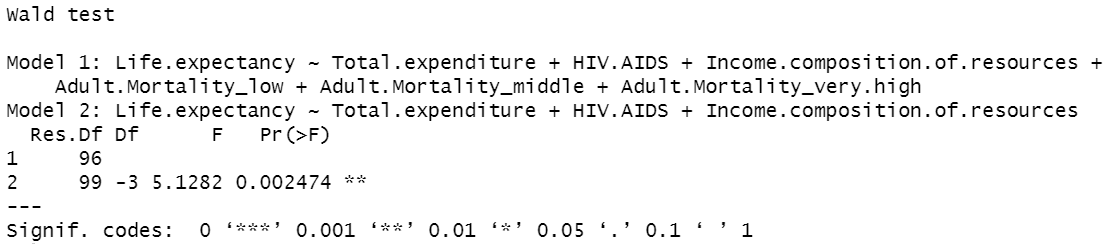
\includegraphics{figures/hypothesis_testing/wald_test_subset_coeff_zero.PNG}
	\caption{Output of Wald test}
\end{figure}

The p-value is 0.0025 which is below the significance level of 0.05. We can thus reject the null hypothesis. We can conclude that there is sufficient statistical evidence that the different categorial variables corresponding to adult mortality rates explain life expectancy. 

\section{Prediction interval}

We calculate a 95\% prediction interval for the 26 observations excluded from the dataset in the beginning. We conclude that almost all the intervals cover the excluded observations. The last observation of the test dataset is the only one not covered by the corresponding 95\% prediction interval. However, if we take the 99\% prediction interval, this observation is contained in the prediction interval.
